\chapter{Organic Reactions Need Not Be Memorized One by One}

\begin{kaichang}
Find three things in the kitchen: an apple, medicinal disinfectant alcohol, and bread in a plastic bag.

Cut the apple and leave it for half an hour. Its white flesh slowly turns an unattractive tea-brown. Meanwhile the alcohol and bagged bread sit quietly, apparently unchanged.

Guess three things: apple browning, alcohol burning, and making a plastic bag seem unrelated, but might they share a language? If a dictionary of thousands of organic reactions lay before you, how many would you need to memorize to count as knowing organic chemistry?

Write down your answers and return at the end. Here is a preview: far fewer reactions may need memorizing than you imagine.
\end{kaichang}

\section{Thousands of Reactions, a Handful of Patterns}

Open a university organic chemistry textbook, and pages of reaction equations, often thousands, can be intimidating. Nineteenth-century chemists did indeed work this way: each new reaction got a name and a notebook entry, like a stamp collection.

Calculate how hopeless stamp-collecting study would be. Over thirty million carbon compounds are known today, with more daily. Even ten common reactions per compound give three hundred million equations. Memorize fifty per day with an extraordinary memory and never a day off, and it takes sixteen thousand years. Clearly no chemist learns this way. Instead, they \textbf{group thousands of reactions into a few families}.

You are already an eyewitness. Bananas turning from green to yellow involve starch breakdown and rewritten flavor molecules; souring milk involves bacteria converting lactose to lactic acid; grilled meat's fragrant browned surface involves hundreds of encounters between sugars and amino acids. Even a perm changes hair by breaking and reconnecting protein disulfide bonds. Their names vary wildly, but at the atomic level they reuse the same actions.

You already have the classification clues. Chapter 36 described carbon frameworks, and Chapter 37 functional groups as reaction interfaces: hydroxyl, carbonyl, carboxyl, carbon--carbon double bonds, each with its temperament. This chapter asks the final question: is there a common script for reactions at these interfaces?

Yes. Its core cast has only three roles, all from our familiar friend, the electron.

\section{Find Electron-Rich and Electron-Poor Sites}

Chapter 11's electronegativity discussion said that when bonded atoms differ, their shared pair favors the more electronegative one. This is not a slogan, but the first foundation for almost all organic reactions.

Take acetone, nail-polish remover's main ingredient. At its center is carbonyl, a carbon--oxygen double bond, \chem{C{=}O}. Oxygen is much more electronegative, pulling the cloud toward itself. Oxygen acquires a little negative charge and becomes \textbf{electron-rich}; carbonyl carbon becomes \textbf{electron-poor}, like someone still hungry. The bond resembles a room with different temperatures at its ends: one crowded, the other empty.

What does that imply? If another electron-rich fragment drifts nearby, where will it go? Like repels like, so it will never approach the already rich oxygen; it heads for electron-poor carbon. Conversely, an electron-poor cation seeks oxygen. Without even naming the reaction, identifying rich and poor sites lets you roughly predict where it starts.

Chemists mark this uneven distribution with $\delta+$, delta plus, at the poorer end, and $\delta-$ at the richer end. These are not full charges, only slight electrical character, yet sufficient for prediction. Try bromoethane's carbon--bromine bond, \chem{C{-}Br}: more electronegative bromine is $\delta-$, carbon $\delta+$. That carbon is the most vulnerable gate, as substitution will soon explain.

The names for these roles sound daunting but mean simple things:

\begin{itemize}[itemsep=2pt]
\item \textbf{Nucleophile}: electron-rich and willing to contribute a pair to form a bond. Negative ions such as hydroxide, \chem{OH^-}, often qualify, as do neutral molecules with lone pairs, such as water and ammonia. Nucleophile means liking to approach a positively charged nucleus.
\item \textbf{Electrophile}: electron-poor and wanting another's pair. Carbonyl carbon and hydrogen ions, \chem{H^+}, are examples.
\item \textbf{Free radical}: Chapter 33's redox discussion mentioned single-electron transfers. Split a covalent bond so each atom takes one electron, and unpaired-electron fragments, radicals, result. They break the pair rule and pass single electrons onward like a relay. Burning, plastic aging, and skin damage sunscreen aims to prevent all involve them. Chapter 39 treats them specifically.
\end{itemize}

Most organic reactions now fit one sentence: \textbf{electron-rich sites seek electron-poor ones; an electron pair moves, an old bond breaks, and a new bond forms}. Molecules have no wishes or intentions. Rather, when pairs flow from higher-energy, less constrained positions to lower ones, the system's total energy falls and change may occur. Chapters 27 and 28's ledger is acting again in organic molecules.

\section{Curved Arrows Show Electrons, Not Atoms}

A script needs notation. Organic chemists use \textbf{curved arrows}, with two often-misunderstood rules:

\begin{itemize}[itemsep=2pt]
\item An ordinary curved arrow with a full head moves \textbf{one electron pair}: its tail begins where the pair currently is, and its head points to the destination.
\item A fishhook half-arrow with half a head moves \textbf{one electron}, specifically for radicals.
\end{itemize}

Try a simple reaction. Pass ethene, \chem{CH_2{=}CH_2}, the gas released during fruit ripening, into hydrogen bromide, \chem{HBr}, and bromoethane forms:

\[\chem{CH_2{=}CH_2} + \chem{HBr} \rightarrow \chem{CH_3CH_2Br}\]

Curved-arrow notation divides it into two steps. First, draw an arrow from ethene's restless $\pi$ electron pair to the partly positive hydrogen of \chem{HBr}; simultaneously, move the whole electron pair of \chem{H{-}Br} onto bromine with another arrow. Second, bromide, now a negatively charged nucleophile with lone pairs, sends an arrow to the newly formed electron-poor carbon, completing the last bond.

Avoid the easiest slip: \textbf{curved arrows record electron accounts, not atomic flight paths}. Real molecules tumble, collide, and vibrate in much messier scenes; no atom flies along your drawn arc. Arrows answer only which pair moved from where to where. Yet clear electron accounts let you derive final atom positions, new bonds, and broken old ones: that is their power.

\section{Seven Families of Organic Reactions}

Classify scripts by how electrons move, and thousands of reactions fit seven families. Each comes with a familiar example.

\subsection{Substitution: One Replaces Another}

An atom or group at one molecular position is replaced by another. A nucleophile arrives with an electron pair to take over, while the former occupant departs with a pair. Some absorbable surgical sutures and Chapter 40's esterification essentially involve substitution. Bleach reacting with organic matter in light also follows substitution, explaining why colored clothes become blotchy after bleach contact.

\subsection{Addition: Open a Double Bond, Add at Each End}

A carbon--carbon double bond's $\pi$ pair is ready nucleophilic ammunition. Meeting an electrophile opens the double bond and attaches a new atom to each end, as ethene adding hydrogen bromide just did. Food-industry hydrogenation turns liquid plant oil into semisolid margarine by adding hydrogen to double bonds, hence hydrogenated vegetable oil on ingredient labels.

\subsection{Elimination: Addition in Reverse}

Remove a small fragment, often water or hydrogen halide, and create a double bond between neighboring carbons. This reverses addition, like replaying the same script backward. Industrial ethene is made in large amounts precisely by eliminating hydrogen from larger hydrocarbons.

\subsection{Oxidation and Reduction in Organic Clothing}

Chapter 33 made clear that redox means electron transfer and changing oxidation numbers, not simply oxygen gain or loss. Organic chemistry nevertheless has a useful shortcut: \textbf{adding oxygen or losing hydrogen} usually means oxidation; \textbf{adding hydrogen or losing oxygen} usually means reduction. Our apple browns as atmospheric oxygen oxidizes phenols; cooking oil becomes rancid through slow oxidation. Viewed from the other side, plant-oil hydrogenation reduces double bonds.

\subsection{Condensation and Hydrolysis: Join and Cut}

Two molecules join into a larger one while releasing water or another small molecule: \textbf{condensation}. Reverse it, using water to cut a large molecule into two parts: \textbf{hydrolysis}. These are life's leading reactions: amino acids condense into proteins, glucose into starch, and digestion depends almost entirely on hydrolysis cutting starch and proteins back into small molecules. Part VI's biological macromolecules brings them repeatedly. Outside life, they are equally busy: nylon and polyester fibers are long chains from repeated small-molecule condensation (Chapter 43). Soapmaking saponification hydrolyzes fats, treated with scents and sourness in Chapter 40.

Again, these seven families are not laws; textbooks classify somewhat differently. They are seven pairs of glasses for seeing order in tangled reactions. Whenever you meet a new one, ask whether electron pairs are doing substitution, addition, elimination, redox, condensation, or hydrolysis. Usually its family becomes immediately clear.

\begin{qiaoliang}
One reactant sometimes gives two or more products. Two accounts already met in Volume I decide the route: the lower \textbf{threshold}, activation energy from Chapter 29, determines the faster path, \textbf{kinetics}; the lower \textbf{destination}, free energy $\Delta G$ from Chapter 28, determines where things finally settle, \textbf{thermodynamics}.

A classic example adds \chem{HBr} to 1,3-butadiene, yielding either an internally double-bonded, lower-energy stable product or a terminally double-bonded product with a lower formation barrier and faster production. Low temperature and short reaction times favor the terminal product: only low walls can be crossed in time, \textbf{kinetic control}. Higher temperature and longer time allow product interconversion, ultimately collecting most material in the deepest energy valley, \textbf{thermodynamic control}.

\begin{center}
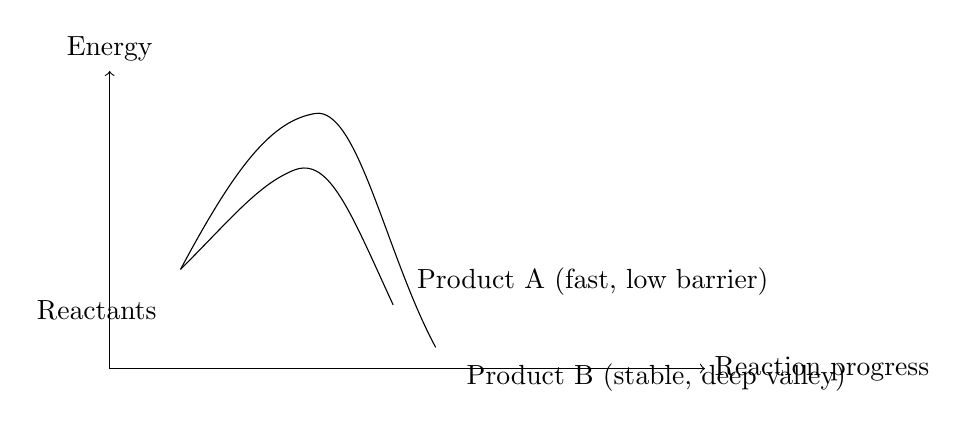
\begin{tikzpicture}[scale=0.9]
\draw[->] (0,0) -- (8.4,0) node[right]{Reaction progress};
\draw[->] (0,0) -- (0,4.2) node[above]{Energy};
\draw (1,1.4) .. controls (1.7,2.1) and (2.1,2.6) .. (2.6,2.8)
      .. controls (3.1,3.0) and (3.4,2.2) .. (4,0.9);
\draw (1,1.4) .. controls (1.8,2.9) and (2.3,3.5) .. (2.9,3.6)
      .. controls (3.5,3.7) and (3.9,1.6) .. (4.6,0.3);
\node at (0.8,1.1) [below left]{Reactants};
\node at (4.2,0.9) [above right]{Product A (fast, low barrier)};
\node at (4.9,0.2) [below right]{Product B (stable, deep valley)};
\end{tikzpicture}
\end{center}

This is a human-made energy schematic, not precisely measured curves. Remember: \textbf{kinetics governs how fast you arrive; thermodynamics, where you stop}. Equating spontaneous with fast, or exothermic with inevitable, mixes the two ledgers, misconceptions already dismantled in Chapters 28 and 29.
\end{qiaoliang}

\section{Mechanisms: Models Bound by Evidence}

You may now feel uneasy: all these confident stories of electron pairs moving, yet nobody saw them relocate. Are curved arrows just rhymes chemists invented?

This is a legitimate challenge, one chemists themselves anticipated. They call the stepwise description a \textbf{reaction mechanism}. A mechanism is a model, not live footage, but a good one must repeatedly pass experiments, explain existing facts, and predict new ones. This classic story shows evidence fastening a mechanism in place.

\begin{zhengju}
Ethyl acetate hydrolyzes to acetic acid and ethanol:

\[\chem{CH_3COOCH_2CH_3} + \chem{H_2O} \rightarrow \chem{CH_3COOH} + \chem{CH_3CH_2OH}\]

The equation looks obvious, but the mechanism has a knot: the ester has two ways to break a carbon--oxygen connection. Does water cleave on the acyl side, giving its oxygen to acetic acid, or on the alcohol side, giving it to ethanol? Both produce exactly the same overall equation, which cannot distinguish them. Identical products, different possible mechanisms: a living example of why an equation is not a mechanism.

The breakthrough came from a special oxygen isotope. Natural oxygen is mainly oxygen-16, with a tiny oxygen-18 fraction carrying two extra neutrons. Its chemical temperament is identical, but Chapter 35's mass spectrometer distinguishes it. In the late 1930s and 1940s, chemists, including work by Polanyi and Szabo, hydrolyzed ordinary esters with \textbf{oxygen-18-labeled water}. Acetic-side cleavage should put labeled oxygen in the acid; ethanol-side cleavage should put it in ethanol.

The result was clear: oxygen-18 entered acetic acid, with almost none in ethanol. Thus the mechanism was pinned down: the acyl--oxygen bond broke and water's oxygen ended in the acid. Today's ester-hydrolysis arrows were established this way. Behind every arrow stands isotope labeling, rate measurements, and intermediate trapping. The method later grew still more powerful: whether photosynthetic oxygen came from water or carbon dioxide was answered with the same oxygen-18 strategy, as Part VI will explain. Mechanisms are models, but \textbf{models dancing in evidence's shackles}. New evidence forces revision.
\end{zhengju}

\begin{shiyan}
\textbf{The Apple-Browning Detective} (safe at home).

\textbf{Materials}: an apple; two clean small plates; half a lemon, or a vitamin C effervescent tablet dissolved in water; a small knife.

\textbf{Procedure}: ask an adult to cut the apple into four slices. Put two untreated slices on Plate A. Put two on Plate B, coating the cut surfaces evenly with lemon juice or vitamin C solution. Leave both uncovered on the table.

\textbf{What to observe}: compare cut-surface color at thirty minutes, one hour, and two hours. You may also compare smells.

\textbf{Safety}: have an adult cut the apple. Eating the experimental slices afterward is not recommended after their long air exposure, not because they became poisonous but because uncovered cut surfaces readily collect microbes.

Lemon-treated apple will brown noticeably more slowly. Browning is \textbf{oxidation} of phenols by atmospheric oxygen, the oxidation family. Lemon juice provides two defenses: vitamin C is an eager reducing agent oxidized ahead of the phenols, while acidity slows the enzyme catalyzing the step. One kitchen comparison combines redox, catalysts, and Chapter 29's rate concepts.
\end{shiyan}

\section{Where Are This Map's Boundaries?}

Seven families and curved arrows make a useful map, but a map is not the territory. Note three clear boundaries in the margin.

First, \textbf{one molecule may have several interfaces}, and conditions determine where reaction occurs. Solvent, temperature, concentration, and acidity can change the dominant product; kinetic versus thermodynamic control is a common tug-of-war. Reading conditions beats memorizing products.

Second, \textbf{some reactions do not follow nucleophile--electrophile scripts}. In one class, several bonds break and form together as electrons relay around a ring, without distinct nucleophiles and electrophiles. You need not master this now; know only that the families cover most common reactions, not all.

Third, \textbf{mechanisms are revised}. Oxygen-18 showed evidence supporting a mechanism; new evidence can equally overturn an old one. Textbooks revise details every few years. Treat a mechanism as the best explanation under current evidence, not doctrine carved in stone. This is the deeper reason against rote learning: remember criteria, not conclusions.

\begin{wuqu}
``Curved arrows trace atoms flying between positions.'' Wrong: they account for \textbf{electron pairs}, not atoms. Atoms in real collisions do not follow those arcs. In nucleophilic substitution, for example, the arrow points from nucleophile to carbon while the displaced group exits from the \textbf{opposite side}. Experiments show complete spatial inversion, like an umbrella blown inside out, called Walden inversion and observed as early as 1893. If arrows were atomic flight paths, this backside entry and exit would be inexplicable.

A related misconception calls radicals rare monsters. Quite the opposite: oxygen itself has two unpaired electrons. Cooking flames, sun-brittled plastic, and rusting iron all involve radical relays. Radicals are not rare; they simply do not follow the electron-pair rule.
\end{wuqu}

\section{Back to the Kitchen's Three Objects}

Now fulfill the opening promise.

\textbf{The cut apple}: browning oxidizes phenols, sending electrons to oxygen while oxidation numbers rise and fall. It belongs to the oxidation family and is enzyme-catalyzed. Chapter 30 showed that catalysts lower barriers without changing the overall ledger. Lemon juice slows it through a reducing agent being oxidized first.

\textbf{The alcohol bottle}: quietly sitting, nothing happens despite ethanol and oxygen's favorable combustion accounts, because the reaction barrier is high. Spontaneous is not fast: Chapters 28 and 29 reappear. A struck match supplies activation energy, and alcohol burns through radicals, Chapter 39's topic.

\textbf{The plastic bag}: it probably comes from ethene molecules adding one after another, opening double bonds and linking head to tail. Thousands of repetitions turn gas into film. This is addition's endlessly repeated version, expanded in Chapter 43's plastics, rubber, and fibers.

Three objects, three changes, none derived from memorizing equations. Polarity shows where electrons are; arrows where they go; families which kind of relocation occurs. The rest is reasoning. Avoiding rote learning means replacing memory with judgment, not being lazy.

\section{From Recognizing Patterns to Planning Routes}

Chemists go further: \textbf{combine patterns into routes}. To make a new drug or biodegradable plastic, reason backward from the target. Condensation last? Substitution before that? Like chess, work backward to purchasable starting materials: retrosynthetic thinking, covered in Chapter 44. Before that, return to the oldest and largest-scale organic reactions, turning underground black liquid into gasoline, diesel, and plastic feedstocks. Burning and cracking feature radical relays rather than electron pairs. Separating petroleum by boiling point, cutting it apart, and recombining it also holds clues to carbon monoxide's toxicity. Chapter 39 starts with that underground black soup.

\begin{tiaozhan}
Why do substitutions differ in speed, and why do some invert configuration? Rate is a detective tool distinguishing two mechanisms. Consider hydroxide replacing halogen in a haloalkane. If experiments show rate depending only on haloalkane concentration, not \chem{OH^-}, only the haloalkane participates in the rate-determining step. It first breaks its carbon--halogen bond into an electron-poor carbocation, then the nucleophile fills the vacancy: unimolecular substitution, SN1. If rate depends on both concentrations, the key step is a backside nucleophile collision with simultaneous old/new bond handover: bimolecular substitution, SN2. Ingold and others established this \textbf{inference of mechanism from rate laws} in the 1930s, a beautiful success for Chapter 29's rule that rate laws come from experiment, not guesswork from equations. Skipping this box does not break the main thread.
\end{tiaozhan}

\section*{Try It Yourself}

\begin{sikaoti}
\item Acetone's carbonyl, \chem{C{=}O}, and ethanol's hydroxyl, \chem{O{-}H}, both contain oxygen. Mark electron-rich and electron-poor atoms in each. Which atom would a negatively charged nucleophile most likely attack in acetone? Explain.
\item Classify these observations among substitution, addition, elimination, oxidation, reduction, condensation, and hydrolysis, explaining each in one electron-relocation sentence: (1) exposed cooking oil turning rancid; (2) ethene ripening green bananas yellow and sweet, remembering that ethene signals starch breakdown into sugars; (3) eaten rice starch becoming glucose absorbed in the small intestine.
\item Explain ``ethene + \chem{HBr} $\rightarrow$ bromoethane'' to a classmate in two curved-arrow steps: which pair moves from where to where? Do these two curved arrows represent bromine and hydrogen flight paths?
\item A reaction mainly gives Product A cold, but more stable Product B after heating longer. Sketch an energy diagram like this chapter's, locating A and B, and explain both outcomes with kinetic and thermodynamic control.
\item Hydrolyze an ester labeled with oxygen-18 on its alcohol-side oxygen using ordinary water. Under the mechanism established here, will the label end in acetic acid or ethanol? Explain.
\item Find advertising claiming vitamin C supplementation preserves eternal youth. Use this chapter and Volume I's redox knowledge to identify oversimplified antioxidant claims. Consider dose, evidence quality, individual variation, and why a body is not an apple on a plate.
\end{sikaoti}
